% version 1.00, date 08/01/17, auteur Florian Leriche
\speaker{\Pierre}
\subsection{} % PAs besoin de titre

\begin{frame}
\frametitle{Relation client au sein du PIC}
	\begin{block}{Outils pour la relation client}
		\begin{itemize}
			\item Implication forte du client ;
			\item Réunions fréquentes.
		\end{itemize}      
	\end{block}
	\begin{block}{Révision du cahier des charges initial}
		\begin{itemize}
			\item Attentes réelles différentes des attentes écrites ;
			\item Changements en cours de projet ;
			\item Contexte client inédit pour l'équipe PIC.
		\end{itemize}      
	\end{block}
\end{frame}


\begin{frame}
\frametitle{La gestion des ressources du PIC UNICEF}
	\begin{block}{Outils pour la gestion des ressources}
		\begin{itemize}
			\item Diagramme de GANTT ;
			\item Scrum Board.
		\end{itemize}      
	\end{block}
\end{frame}


\begin{frame}
\frametitle{Scrum Board}
	\begin{figure}
		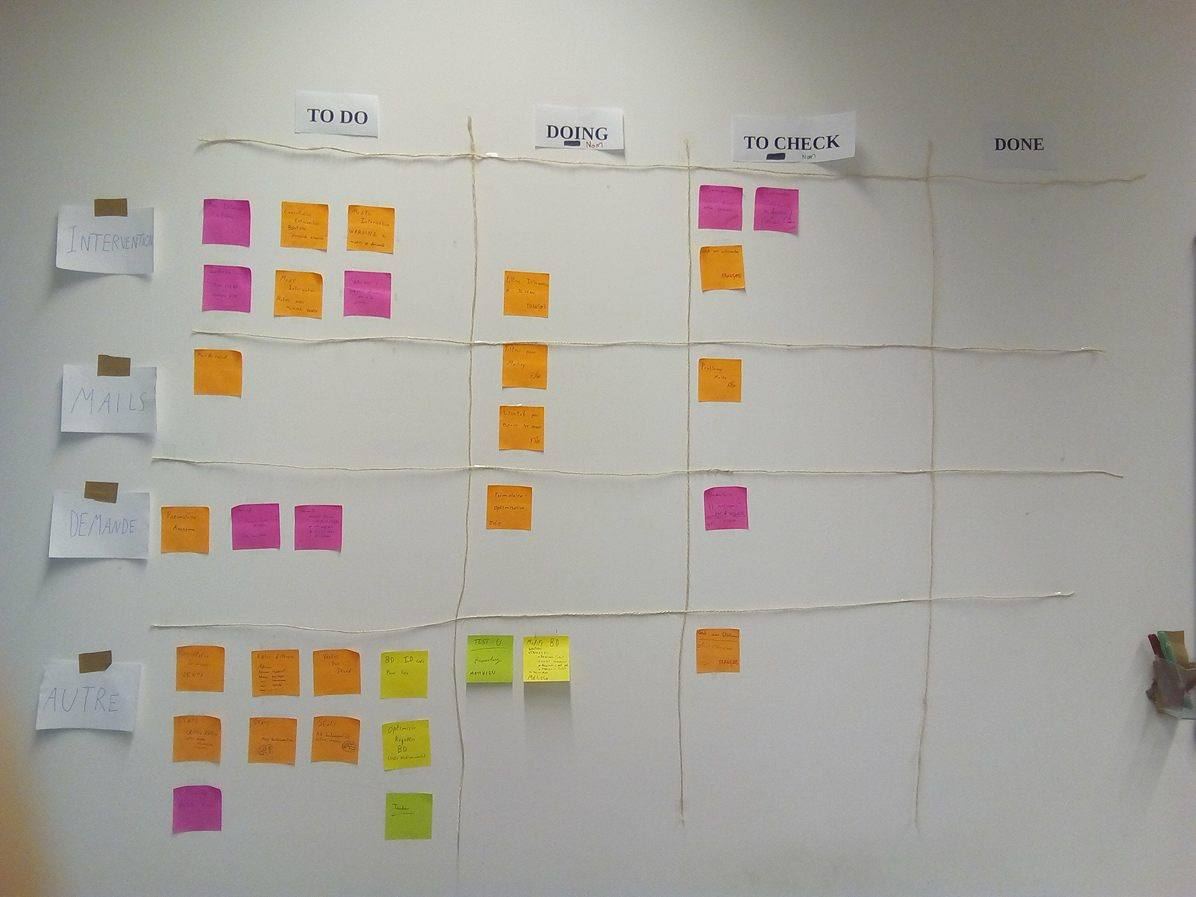
\includegraphics[scale=0.2]{images/kanban.jpg}
		\caption{Notre Scrum Board}
		\label{Kn}
	\end{figure}
\end{frame}
	

\begin{frame}
\frametitle{Retour sur la gestion de projet}
	\begin{block}{Une nouvelle expérience}
		\begin{itemize}
			\item Découverte de la gestion de projet ;
			\item Acquisition de compétences d'ingénieur ;
			\item Dernière livraison le 14 décembre 2016.
		\end{itemize}      
	\end{block}
\end{frame}